\documentclass[10pt,conference,compsocconf]{IEEEtran}

\usepackage{hyperref}
\usepackage{graphicx}	% For figure environment
\usepackage{amsmath}
\usepackage{placeins}
\let\labelindent\relax
\usepackage[inline]{enumitem}
\newlist{inlineroman}{enumerate*}{1}
\setlist[inlineroman]{label=(\roman*)}
\newlist{inlinearabic}{enumerate*}{1}
\setlist[inlinearabic]{label=(\arabic*)}

\renewcommand{\sectionautorefname}{Section}

\usepackage{etoolbox}
\makeatletter
\patchcmd{\@makecaption}
  {\scshape}
  {}
  {}
  {}
\makeatother

\newcommand{\aref}[1]{\hyperref[#1]{Appendix~\ref*{#1}}}

\begin{document}
\title{Investigating classifiers to decode execution and observation processes from intracranial signals}

\author{
  Kolly Florian, Mikami Sarah, Waridel Samuel \\
  \textit{EPFL 2024 | CS433}
  \textit{ML4Science project | TNE Laboratory}
}

\maketitle

\begin{abstract}
    Machine Learning (ML) techniques have become increasingly prominent in neuroscientific research. In particular, many studies investigated the use of ML tools on electroencephalography (EEG) recordings to classify or predict physical and mental states. In this work, we apply ML models to different classification tasks:
    \begin{inlineroman}
        \item Decoding execution from observation
        \item Decoding precision from power grasp in execution paradigm
        \item Decoding precision from power grasp in observation paradigm.
    \end{inlineroman}
    Our work is inspired by ongoing debate over the presence of an action-observation network in cortical signals. By characterizing these signals and applying classification models, we aim to uncover similarities and differences between execution and observation processes in upper limb movements, and to verify whether those characteristics are generalizable across different human subjects. Our findings demonstrate that ML models, including Deep Learning (DL) approaches, can effectively decode execution from observation based on EEG features. However, we also observe that, for tasks where the subject is passively observing different movements, the classical models fail to capture the subtle differences in brain activity and therefore achieve low performances. For show that CNN models show promising outcomes in all classification tasks. These results highlight both the potential and challenges of using ML to decode neural activity using intracranial signals.

%    distinguishing between action execution and observation, and differentiating between precision and power grasps in execution and in observation.
\end{abstract}

\section{Introduction}
Machine Learning (ML) has become a central tool in neuroscience, with applications in neural engineering (e.g. Brain-Computer Interfaces, BCIs \cite{eegforbci}), diagnostics (see \cite{VIEIRA201758} for an overview) and fundamental research (such as the recent NeuroAI field). For instance, Jalilifard et al. \cite{EmotionClassificationSVM} demonstrated the efficacy of Support Vector Machine classifiers in basic emotions recognition, while Bose et al. \cite{EEGRandomForset} used Random Forest classifiers to automate seizure detection in epileptic patients with high accuracy. Indeed, all major ML methods have been applied to neural signals classification \cite{EEGMLReview}.

In this work, we examine the applications of supervised ML models in three classification problems using stereo electroencephalography (sEEG) signals: i) distinguishing between the execution and observation of a movement; ii) differentiating between grasping a small object (precision grasp) versus a large object (power grasp); and iii) differentiating between observing the grasp of a small versus a large object. The sEEG data used here were collected from patients with electrodes in various brain regions. All patients were already implanted as part of their clinical treatment for a drug-resistant form of epilepsy.

% This report describes the data acquisition process, the preprocessing of sEEG signals and the extraction of features. The classical models, as well as CNN, are presented and evaluated on the different classification tasks.

\autoref{sec:analysis} outlines the data acquisition process, the preprocessing of the sEEG signals and the extraction of features. \autoref{sec:actionrecognition} and \autoref{sec:objectrecognition} present the models applied to our classification problems and their performance. In \autoref{sec:deeplearning}, we explore the idea of using only Deep Learning (DL) methods to directly extract features from the sEEG signal and train models. Finally, we discuss our results in \autoref{sec:discussion} and conclude in \autoref{sec:conclusion}.

\section{Data analysis \& preprocessing}
\label{sec:analysis}
The dataset comprises signals recorded from four participants implanted with sEEG electrodes in distinct brain regions as part of their epilepsy treatment. During multiple experimental sessions, participants were instructed to either observe or execute specific motor tasks. These tasks involved two types of movements: a palmar grasp (power-based movement) and a pinch grasp (precision-based movement). Each session included multiple trials. The experimental design is explained in Appendix \ref{subsec:timeline}.

The dataset is a dictionary containing four subjects (labeled \textit{s6}, \textit{s7}, \textit{s11} and \textit{s12}). Each subject participated from one up to three sessions. During each session, the subject completed 256 tasks, equally distributed across observation and execution tasks and across movement types. The number and locations of the channels are not identical across subjects, as they were implanted previous to the experiment.

\subsection{Channel responsiveness}
\label{sec:channelresponsiveness}
We first filtered the channels of interest: for a given channel and task, we define i) the \textit{baseline signal} as the average signal across all task-specific trials in the one-second window between the start of the trial and the cue light turning on, and ii) the \textit{effect signal} as the average signal across all task-specific trials in the one-second equally spaced window surrounding the moment the object is grasped. Using Welch's method \cite{welch}, we computed the power spectral density (PSD) for both the \textit{baseline signal} and the \textit{effect signal}. We then performed a t-test to compare the PSDs and define a \textit{responsive channel} as a channel with a statistically significative t-test (\(\alpha<0.05\), hyperparameter). This analysis was conducted separately for channels responsive during observation trials, execution trials, and responsive to both.

\subsection{Data preprocessing}
\label{subsec:preproc}
The signals of each trial and each channel is preprocessed in three steps:
\begin{inlinearabic}[]
  \item \textbf{Subsampling}: the signal is subsampled from 2048 Hz to 500 Hz to reduce the computational needs. Since the EEG data contains information up to approximatively 150 Hz, this subsampling respects the Nyquist criterion.
  \item \textbf{Z-score correction}: Each EEG signal is normalized with Z-score normalization, calculated using the mean and standard deviation of the \textit{baseline signal}.
  \item \textbf{Resampling}: all trials are resampled to ensure they contain the same number of time points (set to 1500).
\end{inlinearabic}

\subsection{Feature extraction}
Participants with multiple sessions were handled as if they had a larger number of trials. Each task has its own dataset based on the classification task to perform. For action recognition, all trials were taken and labeled as either execution or observation. For movement recognition, trials were taken accordingly to the action type studied and labeled based on the movement type. For all dataset, the features were extracted in a similar way. For each responsive channels of a given task (see \ref{sec:channelresponsiveness}), the trial signal was bandpass-filtered between the following frequency bands: alpha (8-12 Hz), beta (12-30 Hz), gamma (30-100 Hz) and theta (4-8 Hz). For each frequency band, the rectified envelope of the signal was calculated using the Hilbert transform. The trial was divided into segments, each containing 1000 time points. These segments overlapped, with each starting 100 time points after the previous one. The values of one window were summarized using the mean and the standard deviation. Finally, features from each responsive channels, frequency bands and time windows were concatenated in a dataframe.

\section{Action recognition}
\label{sec:actionrecognition}
In this first classification task, we train and optimize different ML models to predict whether the participant was executing the movement or observing it. The analysis is restricted to channels responsive to both movements. Given the distinct nature of the tasks being compared, we anticipate strong performance across all models.

\subsection{Responsivity of channels}
The locations of the responsive channels is critical in understanding a potential action-observation network. To this end, we sorted the responsive channels in ascending order of the t-tests' p-values. For participant \textit{s6}, \autoref{fig:s6actionrecogchannels} shows the locations of the ten first responsive channels, in the precentral and the postcentral gyri. \autoref{tab:actionrecogchannellocations} shows the locations of the most responsive channels for all participants.

The most important regions are similar across participants and are directly linked to movement (ex : prec.) or somatosensory information (ex : postc.). This was expected as the task is linked with active hand movement and requires sensory feedback. It is interesting to note that some of the participants (\textit{s11} and \textit{s12}) have activity in areas that are more related to self-awareness and self-perception (ex: sf. and ins.), which could be much more linked to the observation trials.

\vspace{-1em}

\begin{figure}[h!]
    \center
    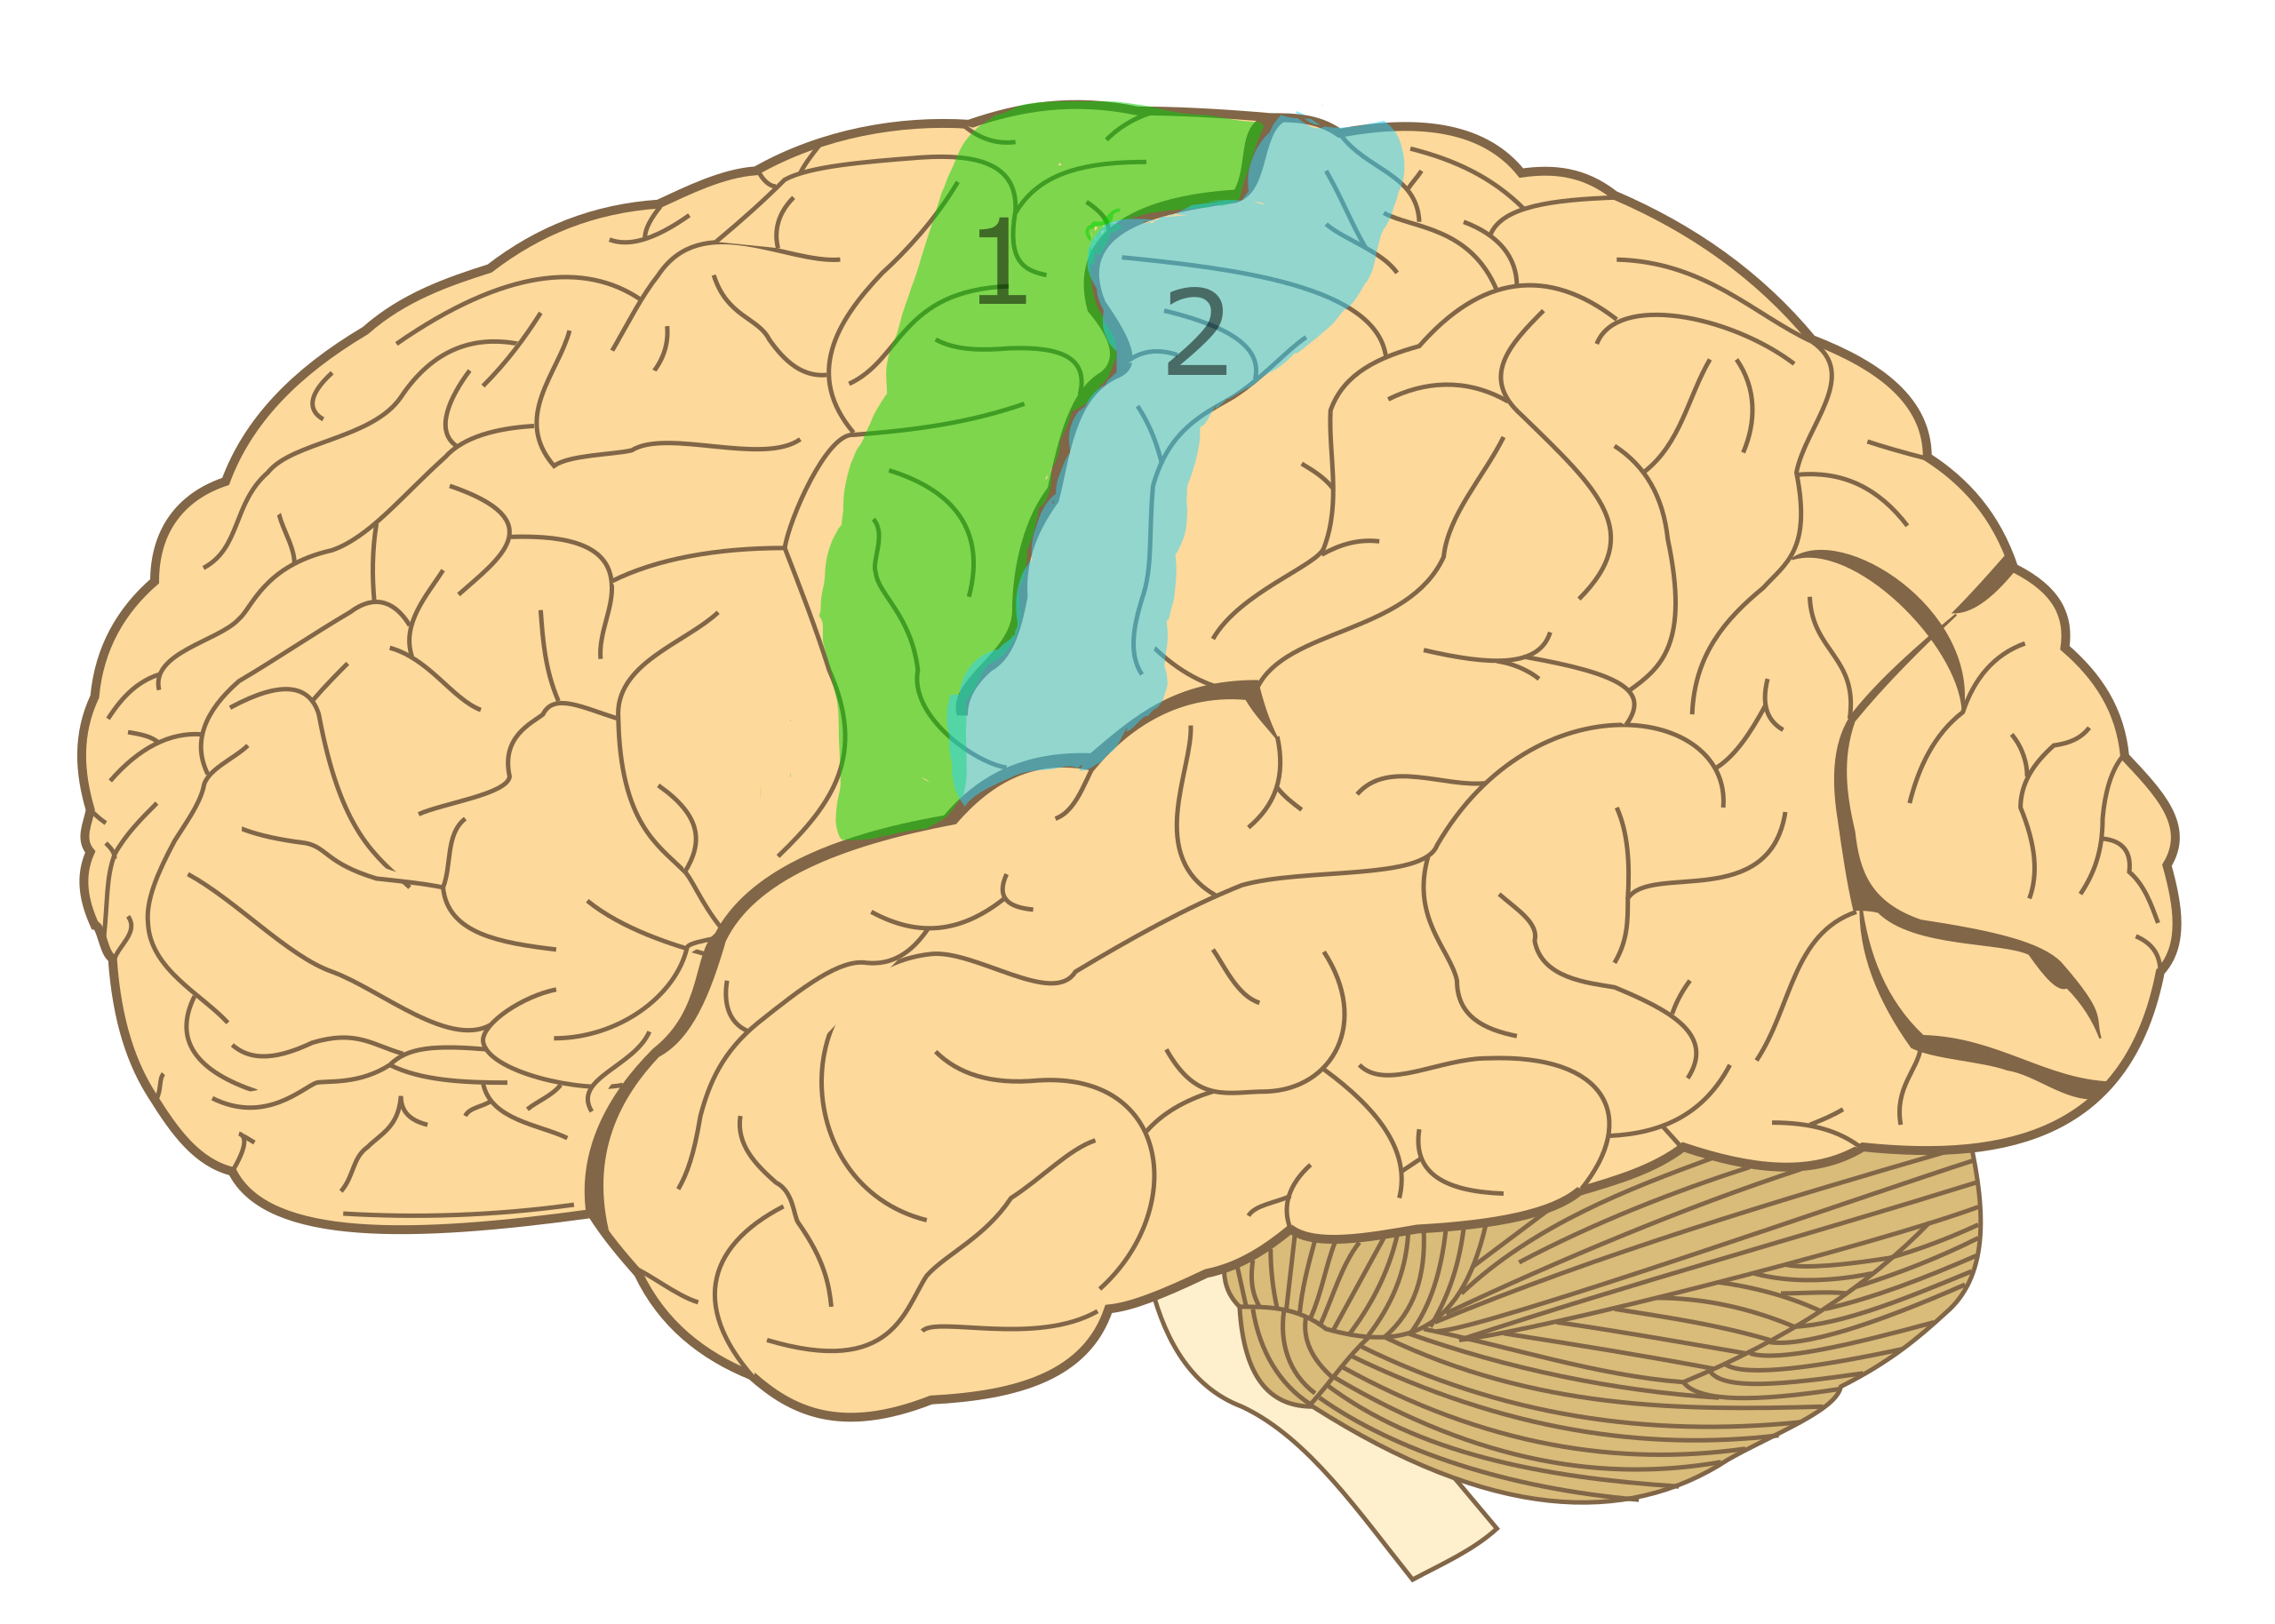
\includegraphics[width=0.7\linewidth]{images/Human-brain.png}
    \caption{Locations of the ten most responsive channels in \textit{s6}: The green area (1) represents the precentral gyrus, and the blue area (2) corresponds to the postcentral gyrus. Edited from Hugh Guiney, CC BY-SA 3.0 \url{https://creativecommons.org/licenses/by-sa/3.0}, via Wikimedia Commons}
    \label{fig:s6actionrecogchannels}
\end{figure}
\FloatBarrier

\begin{table}[h!]
    \centering
    \begin{tabular}{| c | c | c |}
        \hline
        Part. & \# channels & Main locations (\# channels) \\
        \hline
        \textit{s6} & 40 & prec. (5), postc. (5) \\
        \hline
        \textit{s7} & 26 & prec. (7), postc. (1), cmf. (1), parso. (1) \\
        \hline
        \textit{s11} & 27 & prec. (1),  rmf. (1), sf. (5), WMpara. (2), para. (1) \\
        \hline
        \textit{s12} & 29 & ins. (4), sp. (1), pc. (2), para. (1), postc. (2) \\
        \hline
    \end{tabular}
    \caption{Number of responsive channels in total and location of the ten most responsive per participant. \aref{apptab:acronyms} contains the list of acronyms}
    \label{tab:actionrecogchannellocations}
\end{table}

\vspace{-1.5em}
For this task we see that the regions vary quite a bit between participants. Participant \textit{s6} has only two regions with responsive channels, while \textit{s12} has five. The regions with the most importance are similar across participants and are directly linked to movement (ex : prec.)\cite{precentral_gyrus} or somatosensory information (ex : postc.)\cite{postcentral_gyrus}, especially for the first two participants, which is in accordance with the nature of the task. It is interesting to note that some of the participants (\textit{s11} and \textit{s12}) have activity in areas that have weaker ties to motor and sensorimotor functions and perform higher level cognitive tasks (ex: sf. and ins.)\cite{superior_frontal_gyrus}\cite{superior_frontal_gyrus_wikipedia}\cite{insula}, which could be much more linked to the observation trials.

\subsection{Analysis of frequency bands}
We investigate if specific frequency bands could gives more information than other and if there are differences across the action type. We trained the model with a dataset containing only features from a specific frequency band. We then compared the performance of the models across the different frequency bands (see \aref{appfig:accuracies_ExObs_freq_bands}). For action recognition, all models can detect the action type with high accuracy, regardless of the frequency band (above 75\%). The best performance was obtained with delta and gamma frequency bands, with accuracies around 95\%, which suggest that these bands are the most informative for differentiating observation from execution.

\subsection{Baseline data}
To investigate the relevance of selecting only responsive channels, we also generated a list of channels that are not responsive, and computed features from them. We run each model on both sets of data, noting that they have a different number of channels. We discuss only the results of participant \textit{s6}.

\subsection{Models}
To create and train the classical ML models, we adopted the well-known and performant Scikit-Learn library \cite{scikitlearn}. The DL models are developed using the PyTorch library \cite{pytorch}. We selected models based on the literature available on EEG analysis.

\paragraph{Logistic regression}
Logistic regression (LR) is a computationally simple ML technique, and has previously used in EEG classification \cite{SUBASI200587, NIPS2006_35937e34}. It was trained with and without Principal Components Analysis (PCA, 95\% explained variance).

\paragraph{SVM}
We train two Singular Vector Machines (SVM) models, with and without PCA. SVM can handle high dimensional data, even for small datasets. Although more computationally demanding than other methods, it is widely used in EEG classification with good results \cite{knn_svm_review}. We use a grid search to find good hyperparameters for the SVMs (see \aref{subsec:mlhyperparams}).

\paragraph{Random forest}
Random Forest (RF) classifiers are frequently used with a lower set of carefully crafted features (e.g. in \cite{eegrfclassif} with 11 features), we hypothesize that we can also have interesting results using RF here. We use a grid search to find good hyperparameters (see \aref{subsec:mlhyperparams}).

\paragraph{MLP}
In addition to traditional ML models, we also train Multilayer Perceptron (MLP) models. We chose to include MLP as it is widely used in EEG classification\footnote{3'610 results for 'EEG MLP classification' on Google Scholar in 2024}. The main issue with MLP is that they are universal approximators and are thus prone to overfitting, especially for datasets as small as ours.

We try different MLP and select the best by using a validation subset. MLP models are trained for 10 epochs with batches of 4 datapoints. We use the AdamW optimizer, which directly applies weight decay (\(10^{-2}\), hyperparameter) directly during the parameter update, leading to more consistent regularization and better generalization. We use the cross-entropy loss. MLPs are optimized and discussed only for participant \textit{s6}.

\subsection{Results}
We tested the models on the same test set. As expected, all models obtained very high accuracies. When using non-responsive channels, we see a large drop in performance, although it is higher than chance (see \aref{appfig:accuracies_ExObs}). This confirmed our hypothesis that we can reduce significantly the number of features by first selecting responsive channels.

The MLP is performing very well for participant \textit{s6}: on the test set, we obtain an accuracy of 95\% while the baseline is at 49\%. The best model is also the simplest: two layers of 8 neurons each, with a learning rate of \(10^{-1}\).

\begin{figure}[h!]
  \center
  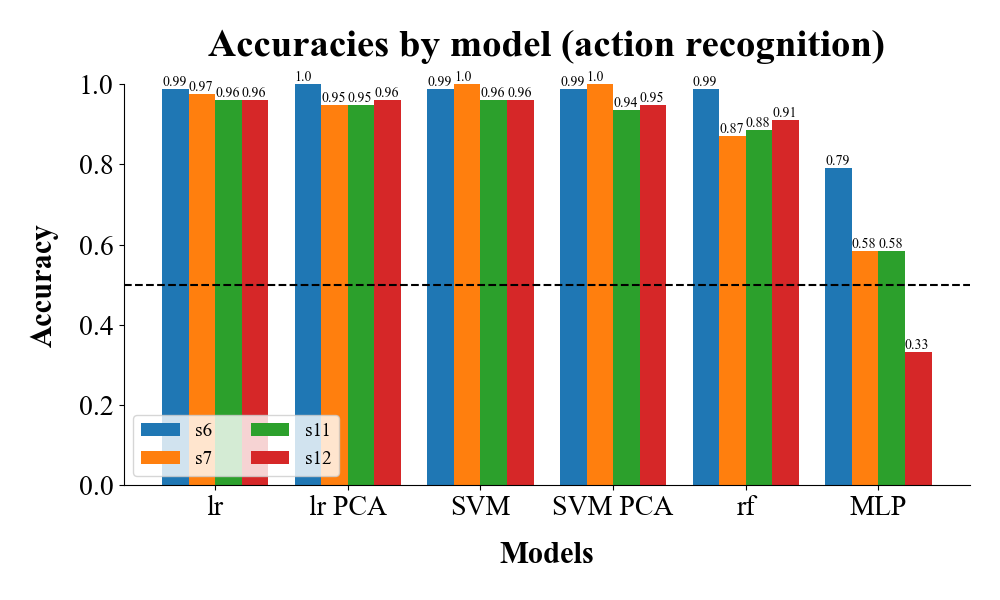
\includegraphics[width=\linewidth]{../Code/figures/accuracies_across_part_ExObs.png}
  \caption{Accuracies by model and participant for the action recognition task: all models perform very well when trained on features extracted from responsive channels}
\end{figure}
\FloatBarrier

\subsection{Analysis of frequency bands}
We investigate if specific frequency bands could give more information than other and if there are differences across the action type. We train the classical models with a dataset containing only features from a specific frequency band. We then compared the performance of the models across the different frequency bands (see \aref{appfig:accuracies_ExObs_freq_bands_freqs}). For action recognition, all models can detect the action type with high accuracy, regardless of the frequency band (above 75\%). The best performance was obtained with delta and gamma frequency bands, with accuracies around 95\%, which suggests that these bands are the most informative for differentiating observation from execution.

\section{Movement recognition}
\label{sec:objectrecognition}
For the second and third type of classification tasks, we analyze whether ML models are able to classify the type of movement done (precision grasp or power grasp) during execution and observation. We expect both tasks to be hard to learn. Observation, in particular, is a complex task, as the participant is simply seeing two different movements that have the same goal of lifting an object. In this part, we lessen the restrictions to select the \textit{responsive channels}: it suffices for a channel to be responsive in execution or in observation respectfully to be included.

\subsection{Responsive channels}
The number of responsive channels and the locations of the ten most responsive channels for each participant are shown in \aref{apptab:exmovchannellocations} for execution and \aref{apptab:obsmovchannellocations} for observation. In both of these tasks, we see similar overall trends between all of the participants as we saw in the action recognition task. Between the action recognition task and the movement recognition task, we see that the regions are quite similar, but the proportions in which they appear changes. For example, the paracentral cortex (para.)\cite{paracentral} is more present in the action recognition task than in the movement recognition task.

\subsection{Analysis of frequency bands}
The models were trained with features extracted from each frequency bands for both execution (see \aref{appfig:accuracies_ex_freq_bands}) and observation (see \aref{appfig:accuracies_obs_freq_bands}). For execution, the models performed slightly better than chance level, with theta and high gamma bands that performed higher than 60\%. For observation, most models are below chance level except for high gamma frequency band, around 52-58\%. The models are not able to capture the differences between the two types of movements with only one frequency band.

\subsection{Models}
We use the same families of model as in the previous part for both execution and observation paradigms. We test the same hyperparameters grid for MLP, although these tasks might be significantly harder.

\subsection{Results}
As expected, our results are significantly lower in those tasks than in the first part.

\paragraph{Execution trials}
(see \ref{appfig:accuracies_across_part_ex}) LR with and without PCA tends to perform better than the other models (56-77\% across participant). The accuracy obtained for SVM with and without PCA is around the same range except for participant \textit{s7} which have accuracies below chance level and RF is around chance level for all participant (46-64\%).

\paragraph{Observation trials}
(see \ref{appfig:accuracies_across_part_obs}) The trends are very similar to execution trials with slightly lower accuracies.

\section{Convolutional approaches}
\label{sec:deeplearning}
Instead of extracting features on the responsive channels before training deep networks, one can ask whether the networks should learn to do that themselves. We explore this question in this section. We train two types of Convolution Neural Networks (CNN) directly on the trial signals. The hope is that the convolutional layers manage to extract important features from the signal, giving it as input to the subsequent MLP. The models won't be optimized as we are focusing on the proof of concept.

In this section, we are not focusing on performance and thus wont optimize models. Instead, we are attempting new techniques as proof of concept. As MLP, we use only participant \textit{s6} in this section. We used only participant \textit{s6}.

\subsection{Models}

The architectures of the CNNs used are detailed in \aref{subsec:cnnarchi}. We are not testing multiple CNN architecture, but use a validation set for the learning rate, weight decay and the subsequent MLP layers.

\paragraph{One-dimensional CNN}
One-dimensional CNNs are composed of kernels that are convolved with a channel's signal directly. As they operate on data in one dimension, the input will be a tensor of size \((N, C, L)\), where \(N\) is the batch size, \(C\) the number of (responsive) channels and \(L\) the fixed length of each trial. This is close to how we computed our features: supposing the same kernel size as the length of our moving averages, we would get the same features if the network learned moving averages too. Given this and the known power of CNNs, we expect this model to have the best performance. The caveat is overfitting, as we have small datasets.

\paragraph{Two-dimensional CNN}
Two-dimensional CNNs are composed of 2D kernels that will operate on multiple channels at the same time. This means that we give as input a tensor of dimensions \((N, C, H, W)\), with \(H\) the number of (responsive) channels and \(W\) the length of each signal. The naming of the dimensions \(H\) and \(W\) is not arbitrary. Indeed, we can think of this superposition of channels as a picture, where each signal is a position on the \(y\)-axis and every timepoint a position on the \(x\)-axis.

\subsection{Results}
The 2D CNN can recognize actions with a 96\% accuracy, while its 1D counterpart has 100\% accuracy. For movement recognition, the 2D CNN manages only 62\% accuracy for execution, with a 92\% accuracy for the 1D CNN. In observation, both models are good, with 77\% accuracy for 2D and 85\% for 1D CNN. Those results are highly encouraging, and we encourage further research towards an automatic way to extract features.

\section{Discussion}
\label{sec:discussion}
All models offered high accuracy in the action recognition task. Interestingly, we observed that our models also performed well even when given features extracted from only one frequency band. The locations of the responsive channels were found to be linked to movement or somatosensation, which corresponds to the experiment.

As expected, both movement recognition tasks resulted in low performance across all the classical models, as well as for shallow neural networks. We hypothesize that this is due to only low differences in the neural signals between the paradigms studied.

However, by approaching the problem from a pure Deep Learning point of view, it appears that convolutional networks are able to themselves extract relevant features for classification. Without hard hyperparameters optimization, we obtained significantly higher accuracy than any other model for the movement recognition task.

\section{Conclusion}
\label{sec:conclusion}
In this project, we used various ML models to analyze the classification accuracies of three distinct tasks. While every model was capable of classifying well the first task, the performance dropped when the differences in brain signals were more subtle. Our work therefore shows that ML models can already successfully be applied to (s)EEG signals without the need for handcrafted features, but they need clear differences in signal. Further experiments can be done on the models developed here to finetune them and verify whether they are able to achieve similar accuracy as in more distinct tasks or not. Additionally, more research is necessary on the preprocessing pipeline and feature extraction as to find optimal data to feed the models. Maybe the future of feature extraction is by using ML methods directly.

\newpage
%%%%%%%%%% ETHICAL RISKS %%%%%%%%%%
%% 200 to 400 words max., does not count in the 4-page limit
\section{Ethical risks}
It is clear that the analysis of EEG and other brain signals present a unique set of ethical challenges. Given that we are not sharing the dataset for privacy concern, we will focus on this ethical risk in this brief analysis. EEG signals reveal information not only about the physical health of a subject, but also mental states, emotions and cognitive functions. With the popularization of such tools, we risk losing a fundamental right to mental privacy. This is not only true for emotions, but also religious and political opinions. For instance, neuropolitics\cite{neuropolitics} is a whole field of research that wishes to find the neural roots of our political beliefs. Prediction is just a step further, step that already stated with work such as \cite{galli_early_2021} and \cite{yun_erp_2022}.

As current methods require possible invasive electrodes, or to use expensive and complicated machines such as fMRI scanners, primarily patients ongoing clinical treatment and study subjects are affected by those risks at the moment. However, the potential violation of cognitive privacy underscores the need for robust privacy and anonymization measures when using EEG datasets. If not correctly established, third parties could gain valuable data on the private mental processes of a user and use it to their advantages. Companies such as Tesla or Meta already invested in such technologies, and not renowned for their privacy-oriented policies. The severity and ramifications of cognitive privacy violating in a large pool of user is hard to quantify, but without strict policies, the possibility of a future without private thought becomes alarmingly plausible.

Even without speculating about future developments in brain signal analysis, EEG signals are already used in identifying individuals. For example, tools for User Authentication via EEG signals already exists\cite{10058960}. It is then clear that, when in possession of private EEG data, precautions must be taken to ensure that this data remains within the restricted pool of authorized researchers who have been granted access. In this project, we were careful not to upload this data on any online repository (e.g. GitHub), and we will not give the dataset to correctors outside the TNE laboratory. Moreover, we did not access any personal information from the participants involved.

Advanced methods exist to encrypt data while allowing computations on it\cite{app11167360}. Unfortunately, the time and scope of this project did not permit the implementation of such technologies.

%% Not in the 4-page limit

\section*{Acknowledgements}
We thank Leonardo Pollina for taking us with him on this project, and for his quick and helpful answers to all our questions.

\newpage

\section{Appendix}
\subsection{Experimental setup}
The participants were asked to keep their hands on the resting positions. The led lights are used both to indicate who will realise the action and to specify which objects has to be grasped. A.) execution trial: the participant must pick the small green ball using a precise pinch grasp. B.) observation trial: the experimenter must pick the large red ball using a power grasp. C.) control action, not used in this project.

\begin{figure}[h!]
    \center
    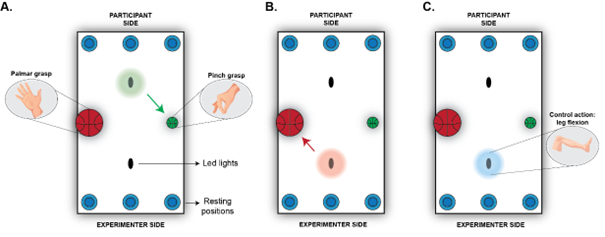
\includegraphics[width=\linewidth]{images/2024-12-11-13-41-23.png}
    \caption{Experimental setup; courtesy of L. Pollina}
\end{figure}
\FloatBarrier

\subsection{Timeline}
\label{subsec:timeline}
Each trial is structured as follows (see \aref{appfig:timeline}): execution trial begins with a start cue. One second later, a light cue signals the type of object (small or large) to be targeted. This light remains illuminated for 0.5 seconds before turning off. After an additional 1.5 seconds, a "go" signal prompts the participant to lift their hand from the resting position, grasp the indicated object, return it to its original location, and place their hand back in the resting position. Observation trials followed an identical structure, except that participants passively observed the experimenter performing the actions. A light cue indicated the participant's role (execution or observation) in each trial.

\begin{figure}[h!]
    \center
    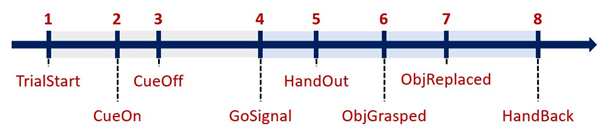
\includegraphics[width=\linewidth]{images/2024-12-11-13-41-48.png}
    \caption{Timing of the trials: the areas shaded in grey indicates fixed timing, and the areas shaded in blue indicates timing that depends on the speed of execution of either the participant (execution) or the experimenter (observation); courtesy of L. Pollina}
    \label{appfig:timeline}
\end{figure}
\FloatBarrier

\subsection{Responsive channels for movement recognition}
Here, we show the locations of the ten responsive channels in the two movement recognition tasks. \aref{apptab:exmovchannellocations} is for the execution tasks, and \aref{apptab:obsmovchannellocations} is for the observation tasks.

\begin{table}[h!]
    \centering
    \begin{tabular}{| c | c | c |}
        \hline
        Part. & \# channels & locations for execution (\# channels) \\
        \hline
        \textit{s6} & 68 & spm. (2), postc. (1), prec. (6), cmf. (1) \\
        \hline
        \textit{s7} & 48 & postc. (1), th. (1), prec. (8)\\
        \hline
        \textit{s11} & 52 & prec. (4), sf. (5), WMpara. (1)\\
        \hline
        \textit{s12} & 76 & para. (1), pc. (3), postc. (2), sp. (1), ins. (3)\\
        \hline
    \end{tabular}
    \caption{Number of responsive channels for execution trials and location of the ten most responsive per participant. \aref{apptab:acronyms} contains the list of acronyms}
    \label{apptab:exmovchannellocations}
\end{table}

\begin{table}[h!]
    \centering
    \begin{tabular}{| c | c | c |}
        \hline
        Part. & \# channels & locations for observation (\# channels) \\
        \hline
        \textit{s6} & 51 & postc. (6), prec. (4)\\
        \hline
        \textit{s7} & 33 & cmf. (1), postc. (2), prec. (7) \\
        \hline
        \textit{s11} & 43 & pren. (1), cmf. (1), para. (1), sf. (6), rmf. (1)\\
        \hline
        \textit{s12} & 48 & para. (2), pc. (3), postc. (1), sf. (1), prec. (1), ins. (2)\\
        \hline
    \end{tabular}
    \caption{Number of responsive channels for observation trials and location of the ten most responsive per participant. \aref{apptab:acronyms} contains the list of acronyms}
    \label{apptab:obsmovchannellocations}
\end{table}

\subsection{Classical models' hyperparameters}
\label{subsec:mlhyperparams}
\paragraph{SVM}
The optimal hyperparameters are found within the following sets using grid search:
\begin{itemize}
    \item \textbf{Kernel}: linear / rbf / sigmoid
    \item \(\mathbf{C}\): 0.1 / 1 / 10 / 100 / 1000
\end{itemize}
\paragraph{Random Forest}
The optimal hyperparameters are found within the following sets using grid search:
\begin{itemize}
    \item \textbf{Number of estimators}: 10 / 50 / 90 / 130
    \item \textbf{Maximum depth}: 10 / 25 / 50
\end{itemize}

\subsection{Acronyms}
\aref{apptab:acronyms} contains the list of brain regions' acronyms used in the report. It does not contain all the regions the participants had electrodes in, but only those relevant in our analyses.

\begin{table}[h!]
    \centering
    \begin{tabular}{| c | l |}
        \hline
        Acronym & Corresponding region \\
        \hline
        cmf. & caudal middle frontal gyrus \\
        ins. & Insula \\
        para. & paracentral \\
        parso. & parsopercularis \\
        pc. & posterior cingulate \\
        postc. & postcentral gyrus \\
        prec. & precentral gyrus \\
	      pren. & precuneus \\
        rmf. & rostral middle frontal \\
        sf. & superior frontal gyrus \\
	      sp. & superior parietal gyrus \\
	      spm. & supramarginal \\
	      th. & thalamus \\
        WMpara. & White Matter paracentral \\
        \hline
    \end{tabular}
    \caption{List of acronyms for the brain regions}
    \label{apptab:acronyms}
\end{table}

\subsection{Accuracies in action recognition compared to baseline}

\begin{figure}[h!]
    \center
    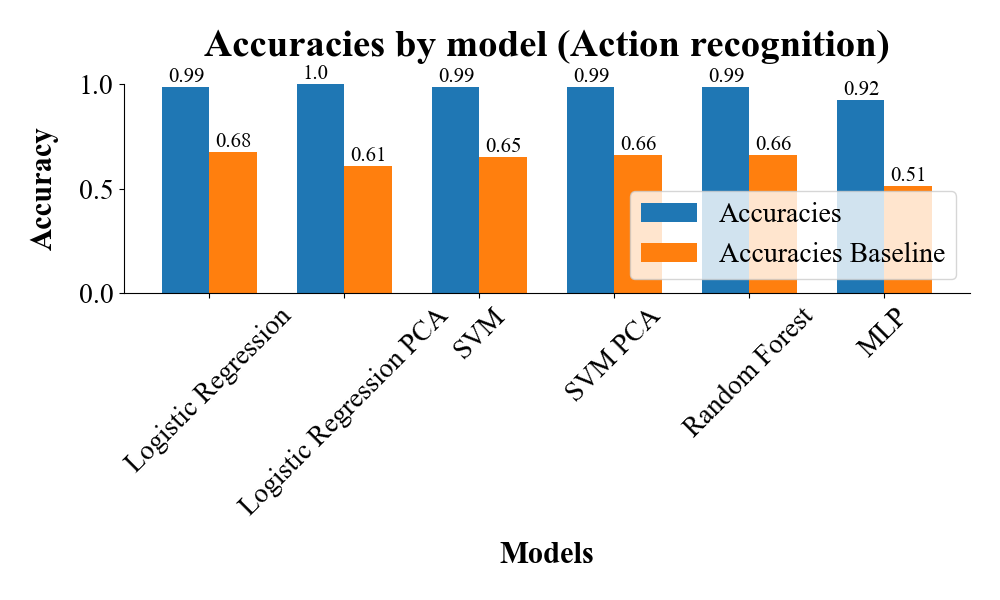
\includegraphics[width=\linewidth]{../Code/figures/accuracies_ExObs.png}
    \caption{Accuracies by model for the action recognition task compared to baseline for participant s6}
    \label{appfig:accuracies_ExObs}
\end{figure}
\FloatBarrier

\subsection{Accuracies in movement recognition}
The following graphs represent the accuracies obtained by model and by participant for the two movement recognition classification tasks. As mentioned in the main report, these accuracies are all low, due to the difficulty of finding neural differences between the compared tasks.

\begin{figure}[h!]
    \center
    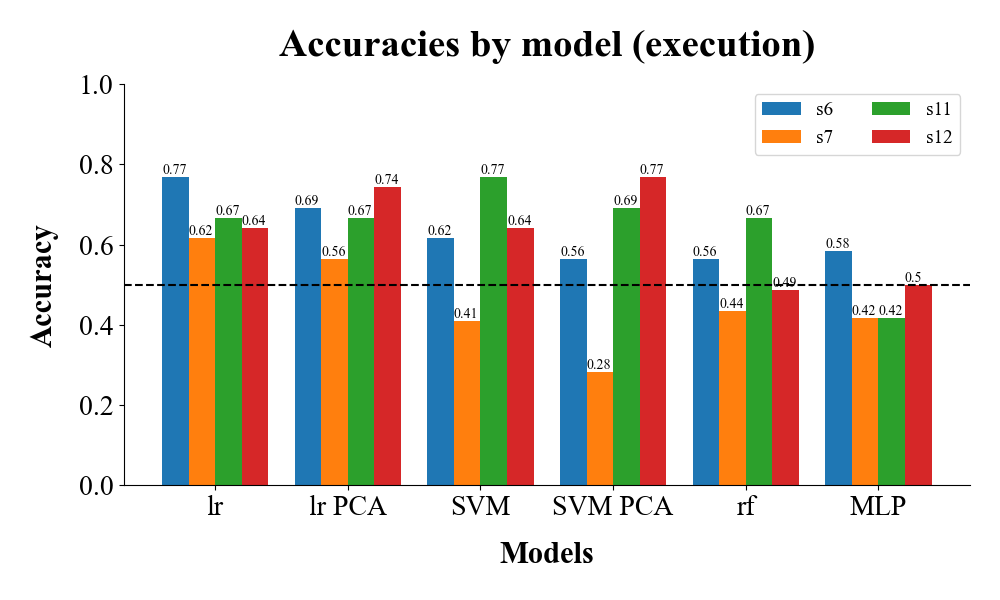
\includegraphics[width=\linewidth]{../Code/figures/accuracies_across_part_ex.png}
    \caption{Accuracies by model and participant for the movement recognition task, executed by the subjects (execution)}
    \label{appfig:accuracies_across_part_ex}
\end{figure}
\FloatBarrier

\begin{figure}[h!]
    \center
    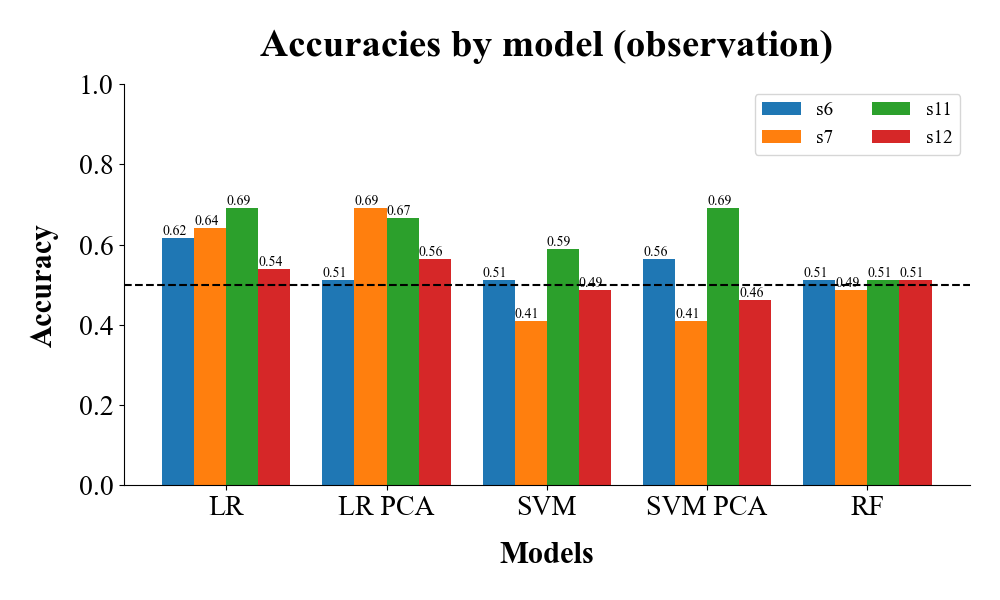
\includegraphics[width=\linewidth]{../Code/figures/accuracies_across_part_obs.png}
    \caption{Accuracies by model and participant for the movement recognition task, executed by the experimenter (observation)}
    \label{appfig:accuracies_across_part_obs}
\end{figure}
\FloatBarrier

\subsection{Accuracies depending on the number of responsive channels}

\begin{figure}[h!]
    \center
    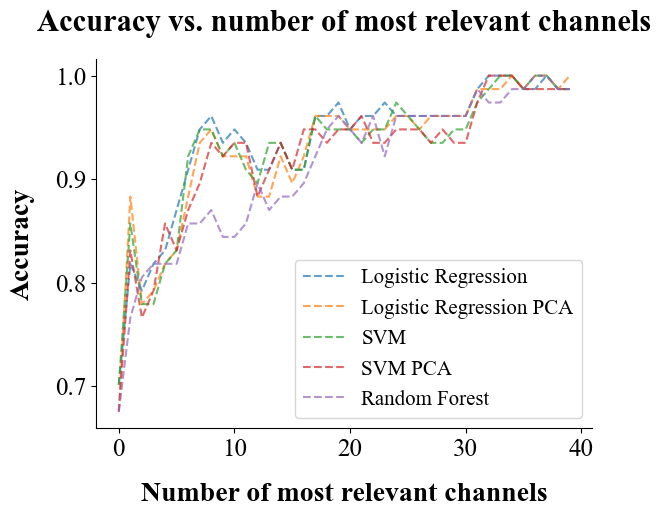
\includegraphics[width=\linewidth]{../Code/figures/s6_acc_vs_channels.png}
    \caption{Accuracies depending on the number of responsive channels used by models for action recognition task on participant \textit{s6}}
    \label{appfig:accuracies_ExObs_freq_bands_channels}
\end{figure}
\FloatBarrier

\subsection{Analysis of accuracy by frequency bands}
Here, we provide an analysis of the accuracies of our model based on which frequency band we give to compute the features.

\begin{figure}[h!]
    \center
    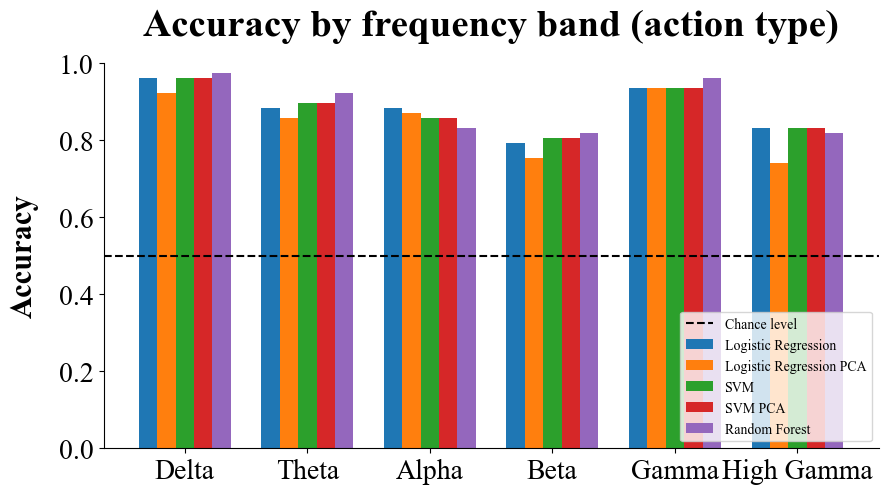
\includegraphics[width=\linewidth]{../Code/figures/s6_accuracies_ExObs_freq_bands.png}
    \caption{Accuracies by model and frequency band used for feature extraction, action recognition task on participant \textit{s6}}
    \label{appfig:accuracies_ExObs_freq_bands_freqs}
\end{figure}
\FloatBarrier

\begin{figure}[h!]
    \center
    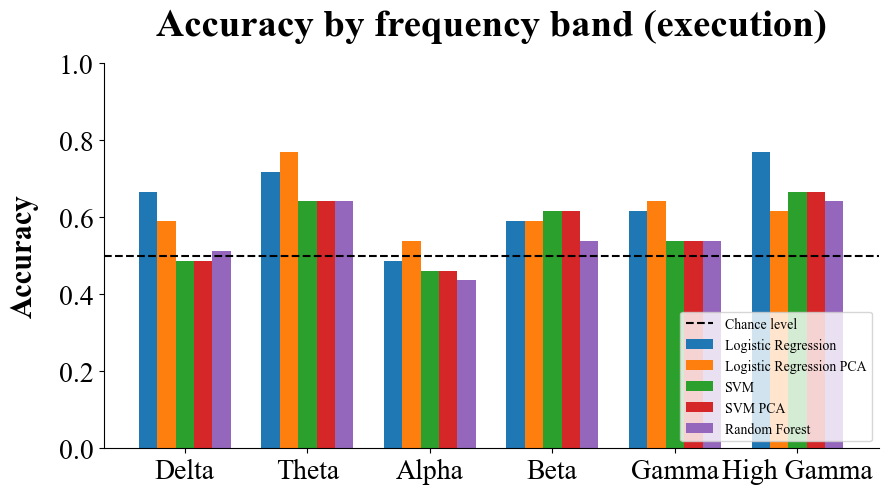
\includegraphics[width=\linewidth]{../Code/figures/s6_accuracies_ex_freq_bands.png}
    \caption{Accuracies by model and frequency band used for feature extraction, movement recognition task on participant \textit{s6} (execution)}
    \label{appfig:accuracies_ex_freq_bands}
\end{figure}
\FloatBarrier

\begin{figure}[h!]
    \center
    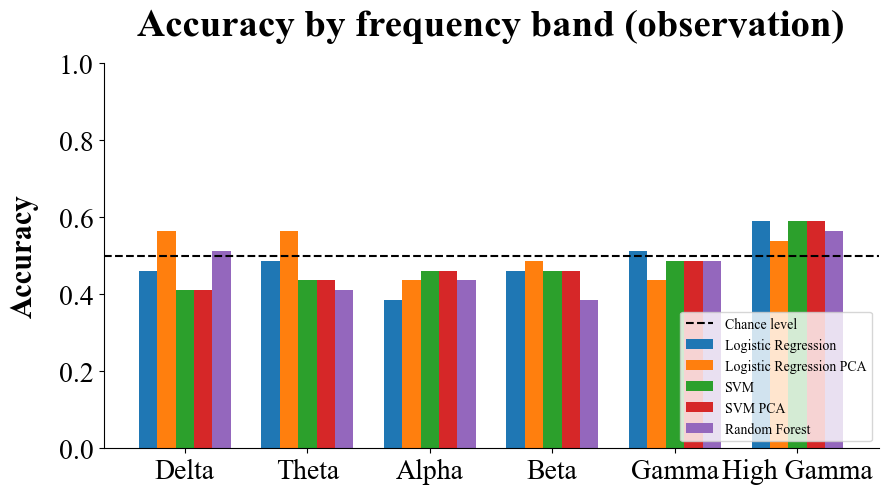
\includegraphics[width=\linewidth]{../Code/figures/s6_accuracies_obs_freq_bands.png}
    \caption{Accuracies by model and frequency band used for feature extraction, movement recognition task on participant \textit{s6} (observation)}
    \label{appfig:accuracies_obs_freq_bands}
\end{figure}
\FloatBarrier

\subsection{CNN architectures}
\label{subsec:cnnarchi}
\paragraph{2D CNNs}
The 2D CNN architecture is as follows:
\begin{itemize}
  \item Convolution layer: 2 channels, kernels of size \(5\times 5\), padding of 1, stride of size \(3\times 3\), ReLU
  \item Max-pooling layer: kernel of size \(2\times 2\)
  \item Batch normalization
  \item Convolution layer: 4 channels, kernels of size \(3\times 3\), padding of 1, stride of size \(3\times 3\), ReLU
  \item Max-pooling layer: kernel of size \(2\times 2\)
  \item Batch normalization
  \item Flattening
  \item Linear layer of 32 neurons, ReLU, dropout of 0.1
  \item Linear layer of 16 neurons, ReLU, dropout of 0.1
  \item Linear layer of 2 neurons, outputs the logits
\end{itemize}
We train all 2D CNNs with a learning rate of 0.001 over 10 epochs with a weight decay of 10 to avoid fast overfitting.

\paragraph{1D CNNs}
The 1D CNN architecture is as follows:
\begin{itemize}
  \item Convolution layer: 8 channels, kernel of size 10, padding of 1, stride of size 5, ReLU
  \item Max-pooling layer: kernel of size 2
  \item Batch normalization
  \item Convolution layer: 16 channels, kernel of size 50, padding of 1, stride of size 5, ReLU
  \item Max-pooling layer: kernel of size 2
  \item Batch normalization
  \item Flattening
  \item Linear layer of 64 neurons, ReLU, dropout of 0.1
  \item Linear layer of 32 neurons, ReLU, dropout of 0.1
  \item Linear layer of 2 neurons, outputs the logits
\end{itemize}
We train all 1D CNNs with a learning rate of 0.001 over 10 epochs with weight decay of 10 to avoid fast overfitting.

\newpage

\bibliographystyle{IEEEtran}
\bibliography{ref}

\end{document}